\documentclass{article}
\usepackage{import}
\subimport{../}{preamble}
\begin{document}

\section{Initial Fabrication of Spherical AuNP-Tipped AFM Probes}
\label{sec:initial_fabrication}

%When aiming to grow a single nanoparticle at the apex of an \gls{afm} tip standard electrodeposition techniques are of little use. The objective of these techniques is to produce an even metallic coating on a substrate electrode rather than growth at a single point. For tips, growth must initially be completely field dependent, taking advantage of the tip's lightning rod effect, but not over sufficient time that smoothing of the apex curvature takes place, reducing the apex field and diverting growth around the resultant neck. Short time-scale, pulsed electrodeposition is investigated as a means of selective nanostructuring.

Selective nucleation and growth of a single nanoparticle at the apex of an AFM tip requires using pulsed electrodeposition, an incredibly uncommon method. The reason for this is that standard methods are designed to produce an even metallic coating rather than growth at a single point. For tips, growth must initially be completely field dependent, taking advantage of the tip's lightning rod effect, but not over sufficient time that smoothing of the apex curvature takes place, reducing the apex field and diverting growth around the resultant neck. By applying a high potential in a short pulse all metallic surface ions are immediately reduced. Charge transfer in this domain can be considered instantaneous and nucleation readily takes place. Accumulation of surface charge therefore does not occur and thus the double layer never forms. Growth in this regime is limited only by mass transport.

\begin{figure}[bt]
\centering
{\fontsize{10pt}{1em}\selectfont \def\svgwidth{0.6\textwidth} \subimport{./figures/}{initial_setup.pdf_tex}}
\caption[Experiment geometry for pulsed electrochemical deposition of Au onto an AFM tip]{\textbf{Experiment geometry for pulsed electrochemical deposition of Au onto an AFM tip.} Electrochemical cell for growth of Au onto the apex of an AFM tip. Termination of field lines at tip apex due to the lightning rod effect enhances localised electrochemical growth for single NP growth.}
\label{fig:initial_setup}
\end{figure}

A simple method is used to successfully demonstrate that a spherical AuNP can be electrochemically grown at the apex of a metallic AFM tip. Conductive coatings are required for the electrochemical reaction, therefore Au- and Pt-coated AFM tips are used (BudgetSensors GB/E series). The adhesion of molecular layers can prevent deposition of Au therefore tips must be cleaned thoroughly prior to deposition. Tips are pre-treated with \SI{20}{\minute} O\subs2 plasma to remove organic contaminants from the surface prior to growth. A simplified two-electrode system (AutoLab PGSTAT 302N potentiostat) is employed for growth since both cell geometry and electrodeposition solution are kept the same between fabrications. AFM probes are attached to fluorine-doped tin oxide (FTO) conductive glass, used as a working electrode, opposite a Pt wire counter-electrode, spaced \SI{10}{mm} apart (\figurename~\ref{fig:initial_setup}). FTO glass is cleaned through sonication in \SI{10}{\minute} steps using \gls{di} water, ethanol and finally acetone. Metalor ECF60 is used as the electroplating solution with no additives. Simultaneous fabrication of both Au and Pt tips can be carried out by contacting multiple tips, closely spaced side-by-side on the same FTO surface.

\begin{figure}[bt]
\centering
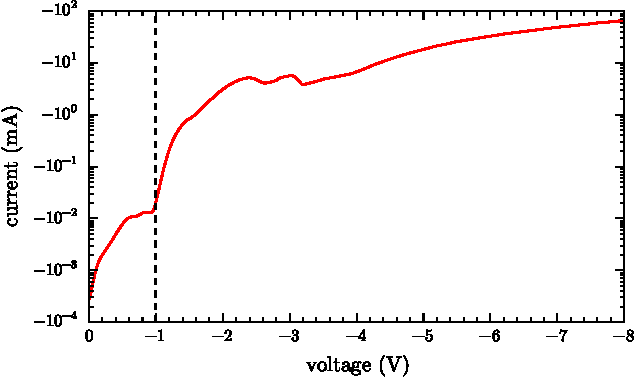
\includegraphics{figures/initial_cv}
\caption[Linear sweep voltammetry of a single AFM cantilever in ECF60]{\textbf{Linear sweep voltammetry of a single AFM cantilever in ECF60.} The AFM probe is held by an Al clamp cathode out of solution, replacing the standard FTO electrode to show growth characteristics of only the tip. The remaining geometry is the same as in \figurename~\ref{fig:initial_setup}.}
\label{fig:initial_cv}
\end{figure}

Linear sweep voltammetry of a single AFM tip in ECF60 (\figurename~\ref{fig:initial_cv}) shows that substantial Au growth starts at around \SI{-1}{V}. This is larger than what is usually expected in ECF60. Differences are attributed to the potentials being referenced to the counter electrode instead of the solution, thus increasing the required potential difference. Further increases in growth are attributed to the activation of water splitting reactions, confirmed by the generation of bubbles at each electrode at higher potentials. An increase from theoretical reduction potentials can also be caused by temperature which factors into the reaction thermodynamics \cite{paunovic2006fundamentals}. The current inevitably becomes limited by mass transport causing the observed saturation at highly negative potentials.

A single high-voltage pulse is applied to nucleate and grow a single AuNP at the tip apex. Due to the large field amplitude at the tip apex, field lines from across the cell terminate at the apex, inducing ions to drift towards the tip apex prior to undergoing reduction (\figurename~\ref{fig:initial_setup}b).  Multiple combinations of applied voltage and pulse times are investigated to optimise growth parameters. Growth of Au onto the AFM tip is confirmed by current dynamics, revealing a 2--\SI{3}{ms} initiation followed by relaxation to continuous diffusion-limited growth within a few 10s of milliseconds. \Gls{sem} imaging, carried out on a LEO GEMINI 1530VP FEG-SEM Scanning Electron Microscope, is used to characterise the resulting growth morphology.

\begin{figure}[bt]
\centering
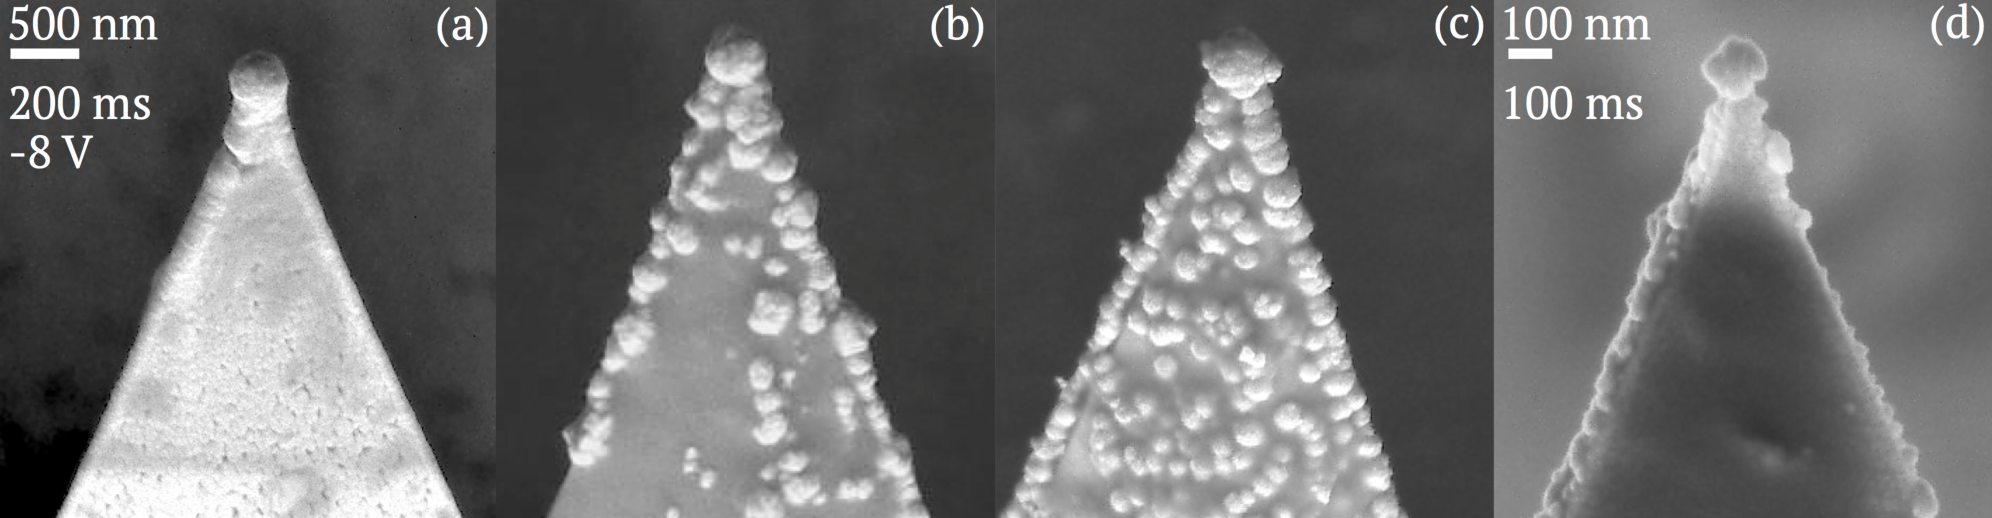
\includegraphics[width=0.9\textwidth]{figures/figure_2}
\caption[Comparison of AuNP-tipped AFM probes, fabricated on various base structures using \SI{-8}{V} pulses of different lengths]{\textbf{Comparison of AuNP-tipped AFM probes, fabricated on various base structures using \SI{-8}{V} pulses of different lengths.} The first three tips were produced simultaneously using a \SI{200}{ms} pulse on (a) a commercial Pt tip with no pre-treatment, (b) a plasma-treated Pt tip, (c) a plasma-treated Au tip. (d) Duplicate spherical tip produced separately on a plasma treated Pt tip using a \SI{100}{ms} pulse.}
\label{fig:electrochemical_tips}
\end{figure}

SEM images of four tip samples fabricated at \SI{-8}{V} are shown in \figurename~\ref{fig:electrochemical_tips}, three of which were fabricated simultaneously on one FTO glass slide, to show the effects of tip pre-treatment and exposure time in the applied field. These images demonstrate that spherical AuNP tips can be reliably fabricated using the proposed electrodeposition procedure. AuNP growth diameters between 150--\SI{450}{nm} are achieved using 100--\SI{200}{ms} pulses across the electrochemical cell on both Pt and Au tips. Evidence of growth localisation to the high field regions is clearly exhibited by the formation of spherical AuNPs at the tip apex. The morphologies obtained differ with and without plasma pre-treatment. Using tips as supplied leads to a smooth sphere at the tip apex, resulting from the lightning rod effect, followed by a broad neck and semi-uniform Au coating across the exposed surfaces of the tip (\figurename~\ref{fig:electrochemical_tips}a). Plasma treatment removes organic contamination and can also oxidise the surface \cite{li2003, fuchs2009}. Removal of contaminants prevents growth at defect sites. The formation of an insulating metal oxide layer prevents growth on surfaces, limiting growth only to sharp regions with a small radius of curvature (\figurename~\ref{fig:electrochemical_tips}b--d). These regions remain conductive and the electric field is large and highly localised. Because Au is more difficult to oxidise than Pt, the shielding effect is different for plasma-treated, Au-coated AFM probes, which exhibit significant localised nanoparticle growth on all exposed surfaces (\figurename~\ref{fig:electrochemical_tips}c). Longer pulse times result in bigger diameters of spherical AuNP, as shown in \figurename~\ref{fig:electrochemical_tips}b and \figurename~\ref{fig:electrochemical_tips}d. A \SI{200}{ms} pulse leads to a spherical AuNP on the Pt tip with a diameter of $\sim$\SI{450}{nm} (\figurename~\ref{fig:electrochemical_tips}b), while the diameter of the AuNP is \SI{150}{nm} with a \SI{100}{ms} pulse (\figurename~\ref{fig:electrochemical_tips}d).

\subsection{Dependence of Tip Morphology on Voltage and Underlying Nucleation Mechanisms}

%Morphology Dependence
\begin{figure}[bt]
\centering
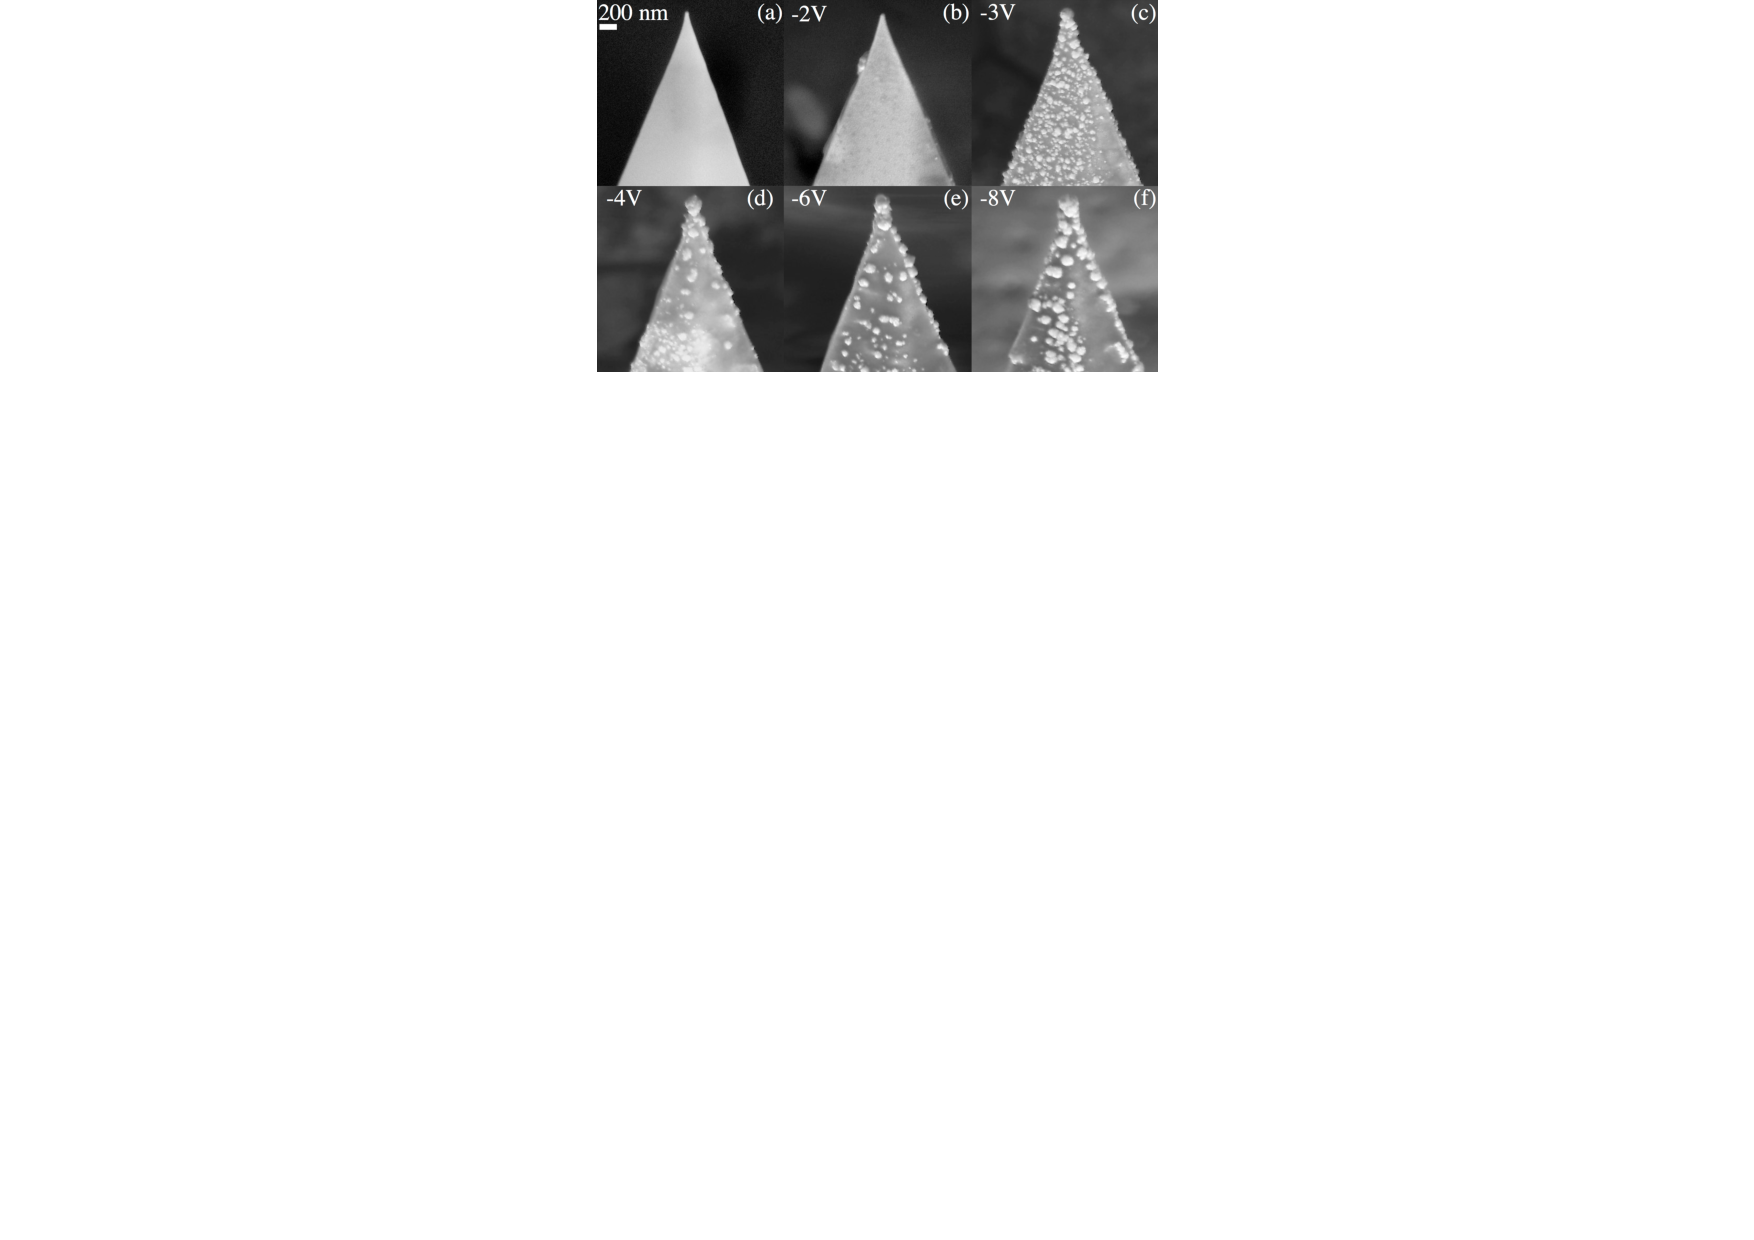
\includegraphics{figures/tip_voltage_dependence}\\
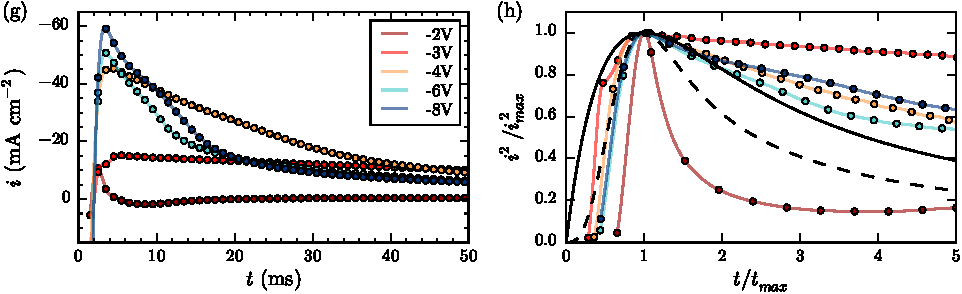
\includegraphics{figures/current_transients}
\caption[Voltage dependence of pulsed electrodeposition onto Pt tips]{\textbf{Voltage dependence of pulsed electrodeposition onto Pt tips.} Comparison between a standard Pt AFM tip (a) and AuNP growth on plasma-treated Pt tips (b-f) using \SI{150}{ms} pulses for voltages between \num{-8} and \SI{-3}{V} and a \SI{500}{ms} pulse at \SI{-2}{V}. This shows the change in deposition mechanism as the magnitude of applied field strength is increased, with no spherical growths above \SI{-3}{V} irrespective of exposure time. (g) Current transients from current traces measured during fabrication of tips shown in (b-f), offset by the saturation current density (\num{-10}, \num{-31}, \num{-34}, \num{-78}, \SI{-142}{\milli\ampere\per\centi\metre\squared}, respectively). (h) Variable-independent reduced current transients (coloured lines) measured at various applied voltages during fabrication compared with theoretical curves for progressive (dashed) and instantaneous (solid) nucleation current transients \cite{scharifker1983}.}
\label{fig:electrochemical_voltage_dependence}
\end{figure}

To investigate the dependence of fabricated tip morphology on the pulsed voltage across the electrochemical cell, the growth of AuNP on Pt tips at different applied voltages is further studied. SEM images of such fabrications along with corresponding current transients are shown in \figurename~\ref{fig:electrochemical_voltage_dependence}. Images show that apex-selected growth occurs only once the voltage is more negative than \SI{-3}{V}. This voltage dependence is attributed to changes in deposition mechanism with field strength.
At low voltages ($V \geq \SI{-2}{V}$), electrodeposition forms smooth film coatings (\figurename~\ref{fig:electrochemical_voltage_dependence}b) similar to direct-current electrodeposition. Under these conditions growth is dominant over nucleation and the field profile caused by the lightning rod effect is eventually evened out, yielding smooth rounded tips. Even with \SI{500}{ms} exposure time no apex-selective growth is observed despite the charge transfer being equivalent to AuNP tip growths at more negative potentials.

%Electrochemical Nucleation Processes
%\begin{wrapfigure}{O}{0.55\textwidth}
\begin{figure}[bt]
\centering
%\vspace{-10pt}
{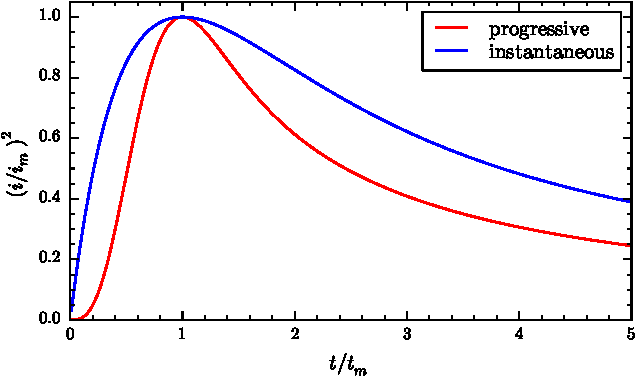
\includegraphics{figures/nucleation_theory}}
{\caption[Reduced current transients for the two extremes of nucleation \cite{scharifker1983}.]{\textbf{Reduced current transients for the two extremes of nucleation \cite{scharifker1983}.} The normalised current, $(i/i_m)^2$, is plotted as a function of time normalised to the maximum, $t/t_m$. Dashed lines show reduced transients from linear transitions between instantaneous nucleation, assuming instantaneous nucleation occurs first then decreases.}
\label{fig:nucleation_theory}}
%\vspace{-10pt}
\vspace{-5pt}
%\end{wrapfigure}
\end{figure}

The electrodeposition morphologies on tips fabricated at potentials more negative than \SI{-2}{V} can be understood to a certain degree by considering it as the boundary for nucleation. Additional insight can be provided by further considering the most common nucleation mechanisms known from AuNP growth on planar electrodes \cite{scharifker1983}. These are progressive and instantaneous nucleation. During progressive nucleation, nuclei form at a time $t$ then grow, increasing the size of the diffusion zone around them, thereby preventing further nucleation within that zone. At the end of progressive nucleation there are many nuclei of different sizes due to the different times at which they each originally nucleated. During instantaneous nucleation all nuclei are formed at $t=t_0$ and then grow at the same rate until their diffusion zones overlap. The overlap of diffusion zones stunts growth as the finite ion flow is split between the two nuclei. For a sparse distribution of nuclei the end result is a set of equally sized particles. For more standard electrodeposition the current transients for progressive and instantaneous nucleation are given in the Scharifker and Hills (SH) model by,
\begin{equation}
\left(\frac{i}{i_{\mathrm{max}}}\right)^2 = \frac{1.2254}{t/t_{\mathrm{max}}} \left[ 1 - \e^{-2.3367(t/t_{\mathrm{max}})^2} \right]^2,
\label{eq:prog_nucleation}
\end{equation}
and.
\begin{equation}
\left(\frac{i}{i_{\mathrm{max}}}\right)^2 = \frac{1.9542}{t/t_{\mathrm{max}}} \left[ 1 - \e^{-1.2564(t/t_{\mathrm{max}})} \right]^2,
\label{eq:inst_nucleation}
\end{equation}
respectively, where $t_{\mathrm{max}}$ is the time at which the current density maximises at $i_{\mathrm{max}}$. {\color{red}Usually the boundary between these two cases is between -0.8 and \SI{-0.9}{V} \cite{}, however this behaviour has not been investigated on short time scales and large, negative potentials where conditions are severely different and the assumptions used to develop the SH model break down.}

% Applying nucleation mechanisms to explain the SEMs
Increased nucleation is observed at \SI{-3}{V} where spherical tip growth is initiated under a progressive nucleation mechanism. Some preferential growth is exhibited at the tip apex but a strong diffusion boundary has not yet formed, as evidenced by the large number of nucleated particles and variation in particle size (\figurename~\ref{fig:electrochemical_voltage_dependence}c). For more negative voltages ($V \leq \SI{-4}{V}$) nucleation becomes more selective, leading to cleaner surfaces and improved apex localisation (\figurename~\ref{fig:electrochemical_voltage_dependence}d-f). This is due to a transition to instantaneous nucleation, in which a fixed number of particles nucleate at selected active sites upon application of a field \cite{hyde2003}. This occurs preferentially at sharp edges where the field is highest. Further selectivity may occur through depletion of ions in the vicinity of the growing tip, preventing additional growth sites. This helps to produce an isolated AuNP at the tip apex. Increasing the magnitude of the voltage increases the number of active sites available for nucleation and more of the tip surface surpasses the field threshold for instantaneous nucleation. Hence, using less negative voltages while still remaining in an instantaneous nucleation regime minimises the number of active nucleation sites, leading to cleaner spherical growth at the tip apex.

% Current transients
A changeover in nucleation mechanisms is also observed in current transients (\figurename~\ref{fig:electrochemical_voltage_dependence}g)%
\footnote{Current measurements are interpolated to create a smooth line through data points. Transients are analysed by first making a quadratic interpolation of experimental data points before data reduction to extract the reduced current transients. This approach is used due to the limited number of points available in the peak region.}
as the shape distinctly changes when decreasing the voltage below \SI{-2}{V}. The largest change in transient shape occurs at \SI{-3}{V}, indicating the onset of shorter time-scale nucleation. Elongation of the transient time is likely caused by contribution to the current from progressive particle nucleation throughout the exposure. Much sharper, short time-scale current transients are observed for potentials more negative than \SI{-4}{V}, supporting the hypothesis of an instantaneous nucleation mechanism as the fast current decay indicates the saturation of all active sites, leaving only diffusion-limited growth.

The influence of instantaneous nucleation for isolated AuNP tip growth is further evident in comparisons to theoretical (SH model) reduced current transients for diffusion-limited progressive and instantaneous nucleation (\figurename~\ref{fig:electrochemical_voltage_dependence}h). Reduced current transients are normalised to $(i/i_{\mathrm{max}})^2$ and plotted against $t/t_{\mathrm{max}}$ to remove variable dependencies, where $i_{\mathrm{max}}$ and $t_{\mathrm{max}}$ represent the peak current and corresponding time. In general, for less negative deposition potentials (\SI{-2}{V}), nucleation resembles more closely progressive nucleation and growth, while at more negative potentials ($V < \SI{-4}{V}$) it resembles more closely instantaneous nucleation. This correlates well with the SEM images shown in \figurename~\ref{fig:electrochemical_voltage_dependence}d-f. Variations from theory occur due to the variable field profile present across the tip leading to localised instances of both progressive and instantaneous nucleation contributing to the overall current. It should be known that the SH model is built upon assumptions such as random nucleation and provides valid results only for the limiting cases of only progressive or instantaneous nucleation, for which the validity fails in such a selectively grown system \cite{dudin2010}.

% More in-depth explanation and model
A simple model can be developed from \gls{sem} images and current transients. Whilst the large surface area of the FTO glass likely dominates the behaviour of the current density, SEM images do indeed show localised changes in the morphology of the tip. When the apex of the tip has a field profile above the threshold for instantaneous nucleation, a single particle may nucleate at the apex and quickly grow. As it nucleates quicker than the rest of the tip its diffusion zone increases to prevent other particles nucleating nearby. This leads to a clean single AuNP growth at the tip apex. If the threshold for instantaneous nucleation is not met then many smaller particles form around the apex (\figurename~\ref{fig:electrochemical_voltage_dependence}c). On the other hand if too much of the tip nucleates instantaneously (very large overpotentials) then the chance for a clean growth is also heavily reduced (\figurename~\ref{fig:electrochemical_voltage_dependence}f) since many particles nucleate around the apex prior to the expansion of substantial diffusion zones. The choice of voltage is therefore imperative to ensuring selective growth of a single AuNP at the apex.

\end{document}